\documentclass[12pt]{article}
\usepackage[margin=1in]{geometry} 
\usepackage{graphicx}
\usepackage{amsmath,amsthm,amssymb}
\usepackage{hyperref}
\usepackage{amssymb}
\usepackage{enumerate}

\title{
    \textbf{Assignment 4} \\ 
    \textbf{AI2000} \\
    \textbf{Foundations of Machine Learning}
}

\DeclareMathOperator{\E}{\mathbb{E}}

\author{
    \textbf{Darpan Gaur} \\
    \textbf{CO21BTECH11004}
}


\date{}

\begin{document}
\maketitle

\hrulefill

\section*{Problem 1}
Consider case of shattering 3 points, $x_1, x_2, x_3$.
Say, $x_1 < x_2 < x_3$, and $x_1$ and $x_3$ are classified as 1.
Give labelling $x_2$ as 0. But as $x_1 < x_2 < x_3$, we can't classify $x_2$ as 0.
Hence, 3 points can't be shattered, so VC dimension is 2.

\section*{Problem 2}
Given, 
\begin{equation*}
    y(x, w) = w_0 + \sum_{k=1}^{D} w_k x_k = x^T w
\end{equation*}
Now adding gaussian noise $\epsilon_k \sim \mathcal{N}(0, \sigma^2)$ to $x_k$:
\begin{equation*}
    y(x, w) = w_0 + \sum_{k=1}^{D} w_k (x_k + \epsilon_k) = (x + \epsilon)^T w
\end{equation*}
Sum of squared loss:
\begin{equation*}
    E(w) = \frac{1}{2} \sum_{i=1}^{N} (y(x_i, w) - t_i)^2
\end{equation*}
Analyzing the effect of noise on $E(w)$, we see expected squared loss, where expectaion taken over $\epsilon$:
\begin{equation*}
    L(w) = \E_{\epsilon} [\frac{1}{2} \sum_{i=1}^{N} ((x_i + \epsilon_i)^T w - t_i)^2] = \frac{1}{2} \sum_{i=1}^{N} \E_{\epsilon} [((x_i^T w - t_i) + \epsilon_i^T w)^2]
\end{equation*}
\begin{equation*}
    \implies
    L(w) = \frac{1}{2} \sum_{i=1}^{N} \E_{\epsilon} [(x_i^T w - t_i)^2 + 2 \epsilon_i^T w (x_i^T w - t_i) + w^T \epsilon_i \epsilon_i^T w]
\end{equation*}
\begin{equation*}
    \implies
    L(w) = \frac{1}{2} \sum_{i=1}^{N} [(x_i^T w - t_i)^2 + 2 \E_{\epsilon} (\epsilon_i^T) w (x_i^T w - t_i) + w^T \E_{\epsilon} (\epsilon_i \epsilon_i^T) w]
\end{equation*}

As $\epsilon_i \sim \mathcal{N}(0, \sigma^2)$, we have $\E_{\epsilon} (\epsilon_i) = 0$ and $\E_{\epsilon} (\epsilon_i \epsilon_i^T) = \sigma^2 I$.
\begin{equation*}
    \implies
    L(w) = \frac{1}{2} \sum_{i=1}^{N} [(x_i^T w - t_i)^2 + w^T \sigma^2 I w]
\end{equation*}

\begin{equation}
    L(w) = \frac{1}{2} \sum_{i=1}^{N} (x_i^T w - t_i)^2 + \frac{\sigma^2}{2} w^T w
    \tag{1}\label{eq:1}
\end{equation}

For $L2$ regularization, 
\begin{equation}
    L(w) = \frac{1}{2} \sum_{i=1}^{N} (x_i^T w - t_i)^2 + \lambda w^T w
    \tag{2}\label{eq:2}
\end{equation}

By comparing \eqref{eq:1} and \eqref{eq:2}, we see that adding gaussian noise to input is equivalent to $L2$ regularization with $\lambda = \frac{\sigma^2}{2}$.

\section*{Problem 3}
\subsection*{Part (a)}
Dendogram for the final result of hierarchical clustering with single linkage is shown in Figure \ref{fig:3a}.
\begin{figure}[h]
    \centering
    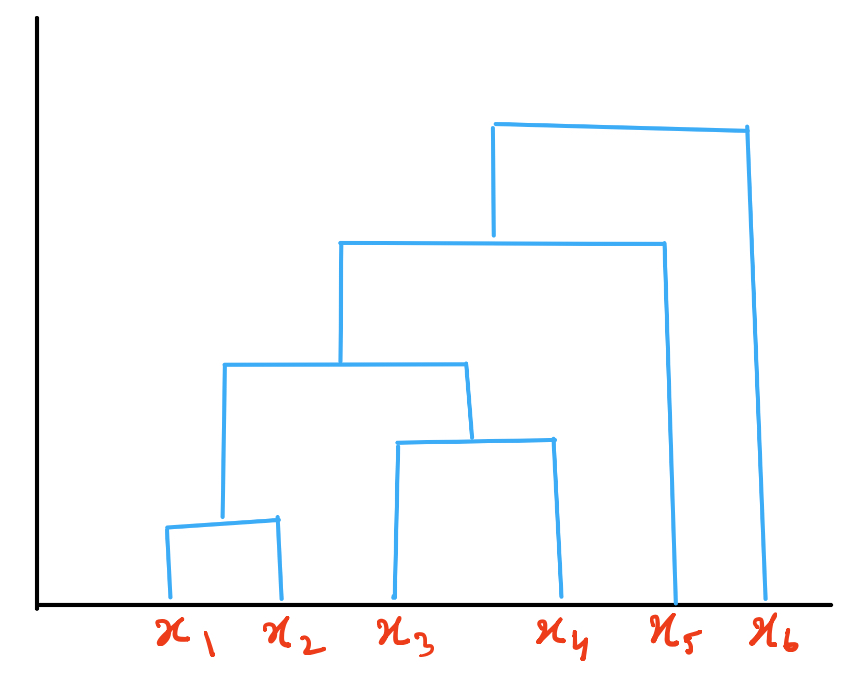
\includegraphics[width=0.5\textwidth]{./images/3a.jpg}
    \caption{Dendogram for hierarchical clustering with single linkage}
    \label{fig:3a}
\end{figure}

\subsection*{Part (b)}
Dendogram for the final result of hierarchical clustering with complete linkage is shown in Figure \ref{fig:3b}.
\begin{figure}[h]
    \centering
    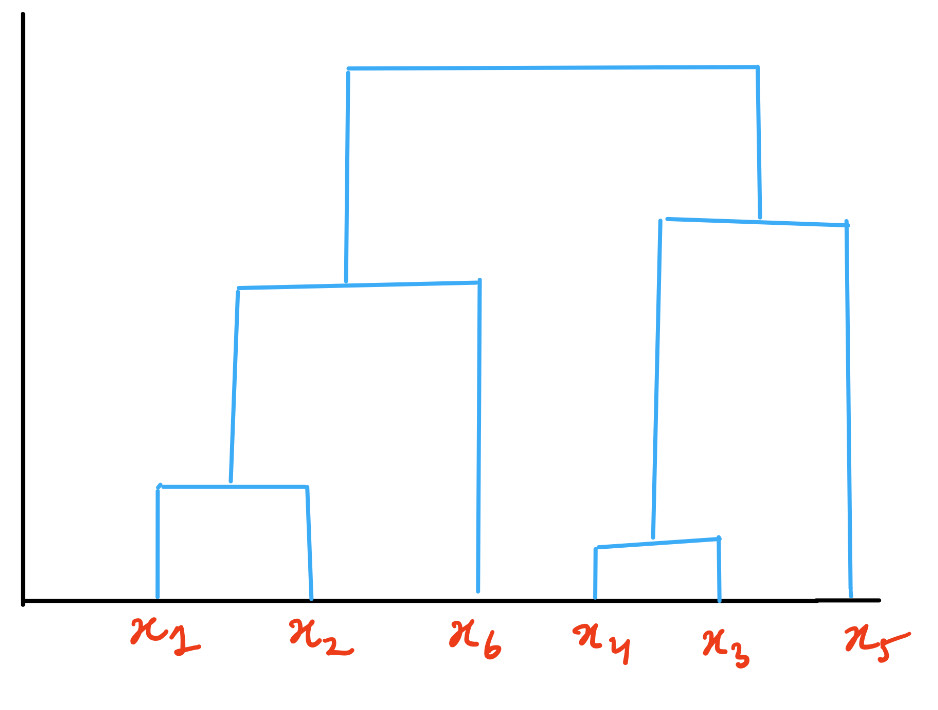
\includegraphics[width=0.5\textwidth]{./images/3b.jpeg}
    \caption{Dendogram for hierarchical clustering with complete linkage}
    \label{fig:3b}
\end{figure}

\subsection*{Part (c)}
Change $dist(x_1, x_2)$ to 0.13 and $dist(x_3, x_6)$ to 0.95. \\
This will not change the resluts of the above question as samll pertubation given to smallest and largest distance, to decrease and increase respectively will not change the results of hierarchical clustering.

\section*{Problem 4}
\subsection*{Part (a)}
\begin{equation*}
    C = \E[(X - \E[X])(X - \E[X])^T]
\end{equation*}
\begin{equation*}
    \implies
    C = \E[XX^T - X\E[X]^T - \E[X]X^T + \E[X]\E[X]^T]
\end{equation*}
As $ x = a\delta_k = a \begin{bmatrix} 0 \\ \vdots \\ 1 \\ \vdots \\ 0 \end{bmatrix} $, where $a$ is scalar and $\delta_k$ is k-th unit vector, distributed over $1, \dots, M$.
\begin{equation*}
    \implies
    C_{ij} = \E[a^2 \delta_i \delta_j^T] - a^2 \delta_i \E[ \delta_j^T] - a^2 \E[ \delta_i] \delta_j^T + a^2 \E[\delta_i \delta_j^T]
\end{equation*}
Two cases arise:
\begin{itemize}
    \item $i = j$:
    \begin{equation*}
        C_{ii} = \E[a^2 \delta_i \delta_i^T] - a^2 \E[ \delta_i ] \E[ \delta_i^T] 
    \end{equation*}
    \begin{equation*}
        \implies
        C_{ii} = \frac{\E[a^2]}{M} - \frac{E[a]^2}{M^2}
    \end{equation*}
    \item $i \neq j$:
    \begin{equation*}
        C_{ij} = - \E[a \delta_i] \E[a \delta_j^T]
    \end{equation*}
    \begin{equation*}
        \implies
        C_{ij} = - \frac{E[a]^2}{M^2}
    \end{equation*}
\end{itemize}
Combinining both cases, we get:
\begin{equation*}
    C = \frac{\E[a^2]}{M}  - \frac{E[a]^2}{M^2} 
\end{equation*}
Gives, $\lambda = - \frac{E[a]^2}{M^2}, \mu = \frac{\E[a^2]}{M}$.

\subsection*{Part (c)}
PCA is not a good way to select features for this problem. \\
This is because, covariance matrix would have one large eigenvalue and $M-1$ small eigenvalues. 
So, variance along the direction of large eigenvalue is large, hence PCA would select that.
But, it may not be the best feature for classification.

\section*{Problem 5}
\subsection*{Part (a)}
Refer to the code in \texttt{5\_logisticRegression.ipynb}.

\subsection*{Part (b)}
\subsubsection*{i} 
Logistic model $P{(\text{y = 1} | x_1, x_2)}$ is given by:
\begin{equation*}
    P{(\text{y = 1} | x_1, x_2)} = \frac{1}{1 + e^{-(\theta_0 + \theta_1 x_1 + \theta_2 x_2)}}
\end{equation*}
Cross entropy loss is given by:
\begin{equation*}
    CE (\theta) = -\frac{1}{m} \sum_{i=1}^{m} y^{(i)} \log{P{(\text{y = 1} | x_1, x_2)}} + (1 - y^{(i)}) \log{(1 - P{(\text{y = 1} | x_1, x_2)})}
\end{equation*}
   
\subsubsection*{ii}
The updated paramters for logistic regression after one iteration are:
\begin{equation*}
    \theta_0 = 1.00316, \theta_1 = 1.50535, \theta_2 = 0.50196
\end{equation*}

\subsubsection*{iii}
At the convergence of gradient descent, metrics are:
\begin{itemize}
    \item Accuracy: 0.67
    \item Precision: 0.6
    \item Recall: 1.0
\end{itemize}

\section*{Problem 6}
Refer to the code in \texttt{6\_house\_prices.ipynb}. \\
Model used and scores on house price prediction are:
% make table
\begin{center}
    \begin{tabular}{|c|c|}
        \hline
        Model & Score \\
        \hline
        CatBoost & \textbf{0.13617} \\
        LightGBM & \textbf{0.14359} \\
        Random Forest & 0.14851 \\
        XGBoost & 0.15374 \\
        Linear Regression & 0.35652 \\
        SVM Regression & 0.41645 \\
        \hline
    \end{tabular}
\end{center}

Top 2 models are CatBoost and LightGBM.

\begin{itemize}
    \item CatBoost: Gradient boosting model, which uses symmetric trees. It is robust to overfitting and can handle categorical features well by using ordered encoding.
    \item LightGBM: Gradient boosting model, which uses leaf-wise tree growth. Uses gradient-based one-side sampling, exclusive feature bundling and histogram-based algorithms. 
\end{itemize}

\begin{itemize}
    \item Random forest and XGBoost also give similar performance as compared to CatBoost and LightGBM. As both similare to them in using ensemble of trees.
    \item Linear regression and SVM regression give poor performance as they are linear models and can't capture non-linear relationships in data.
\end{itemize}

\end{document}